So far, we have looked at different \textbf{supervised learning} techniques:
\begin{itemize}
  \item Decision trees \begin{note}(first categorical, then numerical)\end{note}
  \item Regression \begin{note}(first numerical, then categorical)\end{note}
  \item Support vector machines \begin{note}(SMV)\end{note}
  \item Naive Bayesian classifier
\end{itemize}

All those techniques have the following things in common:
\begin{itemize}
  \item They try to learn a \textbf{function predicting} a \textbf{target} feature in terms of its descriptive features.
  \begin{align*}
    f(\underbrace{\cv{x}}_{\text{descriptive features}}) := \underbrace{\cv{y}}_{\text{target feature}}
  \end{align*}
  \item Some way of measuring the \textbf{error} is provided, e.g. the sum of squared errors, or the number of misclassifications.
  \begin{align*}
    m_{error} : \big\{ (\underbrace{f(\cv{x}_i)}_{\text{predicted label}}, \underbrace{\cv{\hat{y}}_i}_{\text{correct label}}) \big\} \mapsto d \in \mathbb{R}
  \end{align*}
  \item Learning is now based on \textbf{training data}. The evaluation then requires \textbf{test data} (unseen) to address the problem of overfitting.
  \begin{align*}
    \mathcal{D}_{train}, \mathcal{D}_{test} \subseteq \big\{ (\underbrace{\cv{x}_i}_{\text{input}}, \underbrace{\cv{\hat{y}}_i}_{\text{correct label}}) \big\}, \quad
    \mathcal{D}_{train} \cap \mathcal{D}_{test} = \emptyset
  \end{align*}
\end{itemize}

For \textbf{classification} and specifically linear regression and SVMs, we derived the following formula:
\begin{align*}
  y_{\cv{w}}(\cv{x}) = f\left(\sum_{j=1}^M \cv{w}_j\phi_j(\cv{x}) \right)
\end{align*}
\begin{itemize}
  \item $\cv{x}$ is the input vector containing the descriptive features
  \item $\cv{w}$ is our weights vector
  \item The input vector can be lifted to a higher dimension by a mapping $\phi$:
  \begin{itemize}
    \item Simple linear classification: $\cv{x}$ can be used directly
    \item Nonlinear classification: apply feature space mapping or the "kernel trick"\\$\rightarrow$ requires lots of domain knowledge\\$\rightarrow$ increases the number of features $M$
  \end{itemize}
  \item Finally, we see the actual categorizer $f$, which is either:
  \begin{itemize}
    \item A simple threshold-based function with returning $0$ or $1$, or
    \item A more sophisticated function like the sigmoid function \begin{note}(is used in logistic regression)\end{note}
  \end{itemize}
\end{itemize}

We can abstract that further to the following image:
\begin{figure}[H]
  \centering
  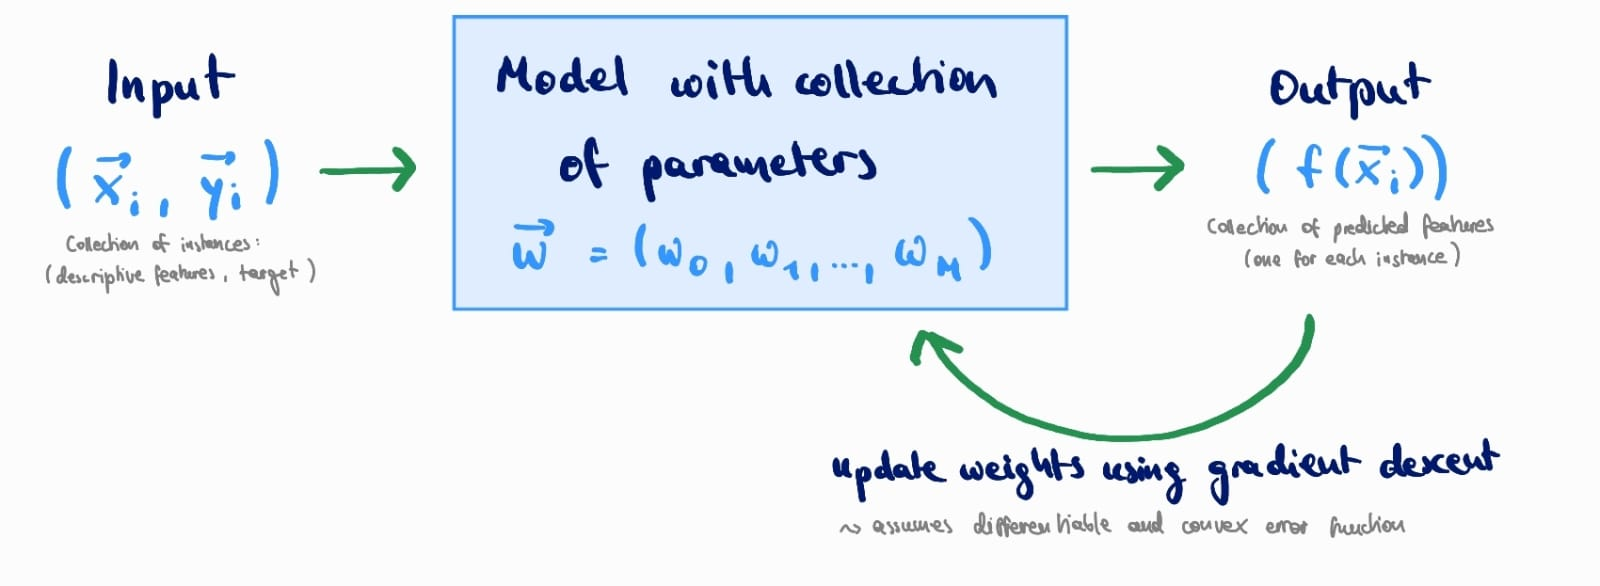
\includegraphics[width=0.7\textwidth]{assets/nn/in__supervised.png}
  \caption{Abstraction on supervised learning}
  \label{fig:6_intro_supervised}
\end{figure}
\begin{itemize}
  \item \textbf{Gradient descent} is a basic principle to iteratively reduce the error by walking down the hill in the steepest direction.
  \item Important is the choice of the step size. If it's too small, the convergence is slow. If it is too large, a risk of overshooting or even divergence arises.
\end{itemize}

Now, the topic of this chapter comes into play: why do we need \textbf{neural networks}?
\begin{itemize}
  \item The input for our classification problem can be anything, e.g. text, sound, images, videos, etc.
  \item This would mean, our classifier can no longer be described by a simple (linear) function.
  \item Our traditional linear approaches don't work anymore. SVM already tried to address this problem by introducing the mapping $\phi(\cv{x})$ to lift the number of dimensions, but this mapping needed to be manually constructed.
  \item In the NN approach: $\phi(\cv{x})$ may be based on other layers and can be learned.
\end{itemize}

Our before-seen function is therefore lifted to the following:
\begin{align*}
  y_{\cv{w}}(\cv{x})[k] = f\left(
    \sum_{j=1}^M w_{jk}^{(2)} \underbrace{
      h\left(
        \sum_{i=1}^D w_{ij}^{(1)} x_i + w_{0j}^{(1)}
      \right)}_{\text{"}\phi_j(\cv{x}) \text{" is now a network}}
    + w_{0k}^{(2)}
  \right)
\end{align*}
\begin{itemize}
  \item We have input $\cv{x}$ with $D$ dimensions or features.
  \item The network uses the activation functions $f$ and $h$.
\end{itemize}

Consider the classification of images with automatic dog detection. For that, many labeled samples (dog and non-dogs) are provided. The samples are pictures, so for the computer just a collection of pixels. This results in a huge number of features. The same can be seen for the example in \ref{fig:6_intro_mnist}. Generally, as the input for our NNs, we're only gonna consider \textbf{unstructured data} such as images, text, sound, or video.

\begin{figure}[H]
  \centering
  \begin{subfigure}{\textwidth}
    \centering
    \begin{subfigure}{0.57\textwidth}
      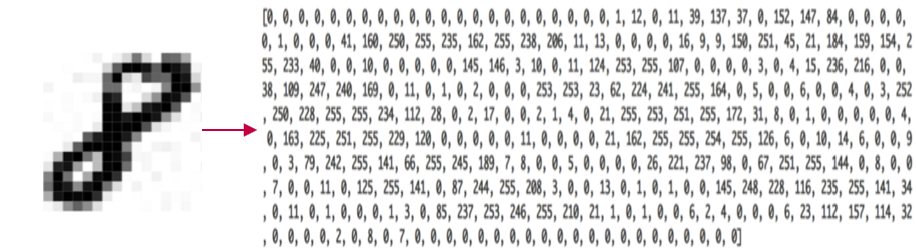
\includegraphics[width=0.9\textwidth]{assets/nn/in__mnist_feature.png}
      \subcaption*{Set of features}
    \end{subfigure}
    \begin{subfigure}{0.33\textwidth}
      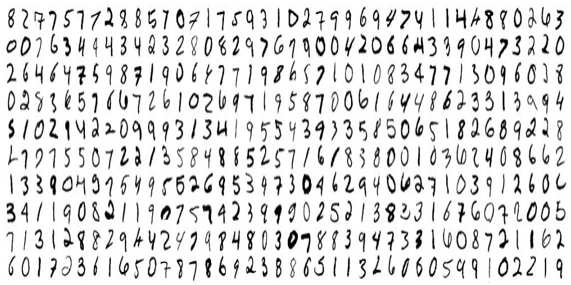
\includegraphics[width=0.9\textwidth]{assets/nn/in__mnist_dataset.png}
      \subcaption*{Training dataset}
    \end{subfigure}
  \end{subfigure}

  \vspace*{0.2cm}
  \begin{subfigure}{\textwidth}
    \centering
    \begin{align*}
    \text{Image} &\ \ =\ \begin{array}{l}\text{grid of numbers representing}\\\text{the darkness of each pixel (grayscale)}\end{array}\\
    \begin{array}{r}\text{Numbers for MNIST are}\\\text{stored as }18\times18\text{ pixel images}\end{array} &\implies \text{Array of }324\text{ numbers}
    \end{align*}
  \end{subfigure}

  \caption{MNIST dataset example (number recognition classifier)}
  \label{fig:6_intro_mnist}
\end{figure}

